% 2010 年重庆卷理科第 6 题：y=sin(ωx+φ) 的部分图象。
% 来源 PDF：普通高考/2010/2010重庆理.pdf，SHA-256 e981a8805207e307d0ec0d8ef50ac0e0cbf93eec9559a29fb88591b483ae0136。
% 原页：第 1 页（A3 三栏）第 1 栏中部，书页码 577。
% 重绘依据（按原页矢量路径换算，横纵同为每单位 24 pt）：
%   曲线自 y 轴上的点 (0,-1/2) 起画，在 x=π/3 处取最大值 1，在 x=7π/12 处与 x 轴相交，
%   一直画到 x=π（恰一个周期，右端回到 y=-1/2）；峰值处画虚线：水平段连到 y 轴、竖段落到 x 轴；
%   x 轴左端伸到 x=-1，y 轴上下均伸出 x 轴。
\begin{tikzpicture}[scale=0.8, semithick]
  % 坐标轴
  \draw[->] (-1.35,0) -- (4.15,0) node[below] {$x$};
  \draw[->] (0,-1.6) -- (0,1.55) node[left] {$y$};
  % 曲线 y=sin(2x-π/6)，x∈[0,π]
  \draw[thick] plot[domain=0:3.14159265, samples=160]
    (\x, {sin(2*\x r - pi/6 r)});
  % 峰值的虚线标注
  \draw[dashed] (0,1) -- ({pi/3},1);
  \draw[dashed] ({pi/3},1) -- ({pi/3},0);
  % 刻度与文字
  \node[left] at (-0.06,1) {$1$};
  \node[below left] at (0,0) {$O$};
  \node[below] at ({pi/3},-0.12) {$\dfrac{\pi}{3}$};
  \node[below] at ({7*pi/12},-0.12) {$\dfrac{7\pi}{12}$};
\end{tikzpicture}
